% ===========================================================================
%  mechanism_split.tex  --  reusable snippet: the multi-flow byte-split mechanism
%  (equal vs throughput-proportional).  \input this into the Design/Mechanism
%  section of the INFOCOM paper (infocom/main.tex) or the thesis.
%
%  REQUIRES in the preamble of the including document:
%     \usepackage[ruled,vlined]{algorithm2e}   % thesis.tex already has this
%     \usepackage{graphicx}
%     \usepackage{amsmath}
%
%  FIGURE FILE:  fig_split_mechanism.pdf  (vector; PNG fallback also emitted).
%     Built by  build_split_mechanism_fig.py  in this folder.
%     If you \input this from a sub-directory (e.g. infocom/), make the figure
%     reachable, e.g. add  \graphicspath{{../}}  or copy fig_split_mechanism.*
%     next to your main .tex.
%
%  FAITHFUL TO  sim.py::run_ring_transfer_proportional  (proportional) and
%  add_ring_neighbor_flows + FlowLevelSimulator.step (equal baseline).
% ===========================================================================

% ---------- Algorithm 1: the two policies, one differing block -------------
\begin{algorithm}[t]
\DontPrintSemicolon
\SetKwInOut{Input}{Input}
\Input{ring edge $e$; message $B$ bytes; $k$ flows; window $W$; step $\mathrm{d}t$}
\tcp{open $k$ sub-flows: distinct 5-tuples $\Rightarrow$ ECMP paths}
\For{$j \leftarrow 1$ \KwTo $k$}{
  $\mathit{sport}_j \leftarrow \mathit{base} + 100\,e + j$\;
  $\mathit{path}_j \leftarrow \textsc{EcmpHash}(\mathit{src},\mathit{dst},\mathit{sport}_j)$\;
  $b_j \leftarrow B / k$ \tcp*{equal init (both policies)}
}
\While{$\sum_{j} b_j > 0$}{
  \ForEach{active flow $j$}{
    $r_j \leftarrow \textsc{MaxMinShare}(\mathit{path}_j)$\;
    $b_j \leftarrow b_j - r_j\,\mathrm{d}t$ \tcp*{drain at fair-share rate}
  }
  \tcp{{\bfseries proportional only} -- re-divide remaining bytes $\propto$ rate}
  \If{window elapsed $\ge W$ \textbf{and} $\sum_{j} r_j > 0$}{
    $\mathit{rem} \leftarrow \sum_{j} b_j$ \tcp*{$\mathit{rem}$ is conserved}
    $R \leftarrow \sum_{j} r_j$\;
    \ForEach{flow $j$}{ $b_j \leftarrow \mathit{rem}\cdot r_j / R$\; }
  }
}
\caption{One multi-flow ring edge. \textbf{Equal split} (baseline) keeps the fixed
$b_j=B/k$ and \emph{omits} the final \textbf{if}, so the slowest flow straggles and
the edge waits for it. \textbf{Throughput-proportional split} re-divides each
window's remaining bytes in proportion to the measured fair-share rate $r_j$
(conserving $\mathit{rem}$), so all $k$ flows finish together. Faithful to
\texttt{sim.py::run\_ring\_transfer\_proportional}.}
\label{alg:split}
\end{algorithm}

% ---------- Figure: the same decision, made visible ------------------------
\begin{figure}[t]
  \centering
  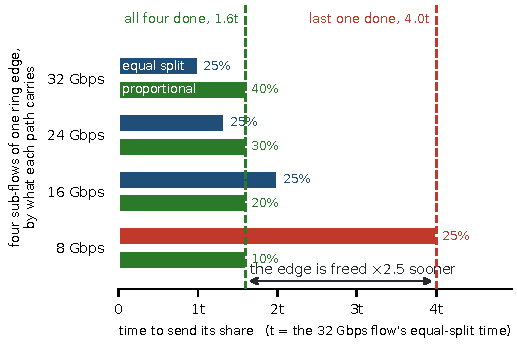
\includegraphics[width=\linewidth]{fig_split_mechanism}
  \caption{How each flow's byte-share is chosen (exact toy: one ring edge, $k=4$
  flows whose measured fair-share rates $r_i$ are $100/50/25/100$~Gbps). Bar length
  is the assigned share. \emph{Equal} split gives every flow $B/k$, so the
  $25$-Gbps flow straggles and the edge waits $4.0t$; \emph{proportional} split
  gives bytes $\propto$ rate ($\tfrac{4}{11},\tfrac{2}{11},\tfrac{1}{11},\tfrac{4}{11}$
  of $B$), so all flows finish at $1.45t$ ($\times2.75$). Here $r_i$ is the
  max-min fair share of Algorithm~\ref{alg:split}.}
  \label{fig:split-mechanism}
\end{figure}
